\chapter{Hierarchical Rule Extraction from Alignment Posterior Probabilities}
\chaptermark{Rule Extraction from Posteriors}
\label{chap:extractionFromPosteriors}

%TODO remove all latex compilation warnings
%TODO somewhere in the introduction, use the convention source and target.
State-of-the-art SMT systems usually decouple word alignment and rule
extraction. This chapter describes rule extraction from alignment posterior
probabilities~\citep{degispert-pino-byrne:2010:EMNLP}. We attempt to extract a
grammar and estimate a translation model that leads to translation improvements.
Grammar extraction and translation model estimation are both based on statistics
given by an HMM alignment model.

This chapter presents two rule extraction methods. With the first method, rules
are extracted from alignment \emph{link} posterior probabilities. With the second
method, rules are extracted from alignment posterior probabilities
over phrase pairs. We
demonstrate improvements on a medium scale Chinese-English task with these
methods. We also investigate how to best exploit source-to-target and
target-to-source alignment models.

\section{Introduction and Motivation}
\label{sec:extractionFromPosteriorsIntro}

In state-of-the-art SMT systems, rules are extracted from a % TODO(check abbr)
word-aligned parallel text where the alignments are generated by the Viterbi
algorithm in the case of Model 1, Model
2~\citep{brown-dellapietra-dellapietra-mercer-1993} or the HMM
model~\citep{vogel-ney-tillmann} or by an approximation to the Viterbi algorithm
in the case of IBM Model 4~\citep{brown-dellapietra-dellapietra-mercer-1993}.
Additional information that these models could provide, such as posterior
probabilities over alignment links, is not used. This work uses HMM alignment
models to generate the statistics needed to both extract rules and estimate the
translation models. We hypothesise that this tighter coupling between alignment
and translation models will provide better translation quality.

We will evaluate the grammar we obtain in two ways. First, we will assess the
grammar's ability to generate a reference translation from a source sentence.
This is determined by the type of reordering allowed by the grammar and by
the choice of translations for each source side of a rule. We will then evaluate
translation quality provided by this grammar.

Conceptually, our extraction method consists in extracting all possible phrase
pairs and hierarchical phrase pairs given a sentence pair and select only the
ones that verify certain statistical criteria related to alignment posterior
probabilities. For example, we can select phrase pairs that contain a link with
a high posterior probability; or we can select phrase pairs that contain a link
with a high posterior probability and that have a high phrase pair posterior
probability. The selection process determines which rules the grammar will
contain and will therefore define the ability of the grammar to generate a
reference translation given a source sentence. We can also use statistics from
alignment models to estimate translation models in a novel way. In this work, we
will use phrase pair posterior probability instead of integer counts to estimate
translation models.

\section{Related Work}
\label{sec:extractionFromPosteriorRelated}

The limitations of extracting translation rules from Viterbi alignments, i.e.
that potentially useful information from the alignment models is ignored, has
been addressed previously. \citet{venugopal-zollmann-smith-vogel:2008:AMTA}
extract rules from
$n$-best lists of alignments and $n$-best lists of syntactic parses for a
syntax-augmented hierarchical system~\citep{zollmann-venugopal:2006:WMT}. They
approximate the posterior probability of an alignment by normalising the
$n$-best list of alignments obtained by the Viterbi algorithm and similarly for
the parses. Rules are then extracted from the cross product of $n$-best
alignments and $n$-best parses and given a count defined in terms of the
approximate posteriors. Alignment $n$-best lists are also used to create a
structure called weighted alignment matrix that approximates alignment link
posterior probabilities, from which phrases are extracted for a phrase-based
system~\citep{liu-xia-xiao-liu:2009:EMNLP}. Our work is very similar, however we
do not use approximations for link posterior probabilities and we apply this
technique to a hierarchical phrase-based translation system.

Alignment link posterior probabilities without approximation have also been
used. \citet{kumar-och-macherey:2007:EMNLP} replace the Viterbi
decision by the maximum a posteriori decision in order to combine word
alignments with a bridge language--for example, Spanish is a bridge language
between Arabic and English if Arabic-English word alignments are derived using
Arabic-Spanish and Spanish-English word alignments.
\citet{deng-and-byrne:2008:ASLP} first extract phrases using Viterbi
alignments and, if test source phrases are not extracted, they extract
additional phrase pairs according to their posterior probability. Our definition
of phrase pair posterior probabilities and the way to compute them are directly
inspired by their work. In this work, our extraction method does not rely on the
Viterbi extraction method, furthermore, we extend it to extraction of
hierarchical phrase-based grammars.

We also note approaches to tighter coupling between hierarchical phrase-based
grammars and alignments or even direct modelling of phrase alignment.
\citet{marcu-wong:2002:EMNLP} introduce a joint phrase-based model that
does not make use of alignments.
\citet{denero-klein:2008:ACL} prove that phrase alignment is an
NP-complete problem. \citet{saers-wu:2009:SSST} report an
improvement on a phrase-based system where word alignment has been trained with
an inversion transduction grammar rather than IBM or HMM models.
\citet{pauls-klein-chiang-knight:2010:NAACL} also use an
inversion transduction grammar to directly align phrases to nodes in a
string-to-tree model. Bayesian methods have also been developed to induce a
grammar directly from an unaligned parallel
corpus~\citep{blunsom-cohn-osborne:2008:NIPS,blunsom-cohn-dyer-osborne:2009:ACL}.
Finally, \citet{Cmejrek2009} extract rules directly from
bilingual chart parses of the parallel corpus without using word alignments.
We take a different approach in that we aim to start with very strong alignment
models and use them to guide grammar extraction.

Finally, another possible direction for better estimation of a translation model
is smoothing, which could be complementary to the approach taken here.
\citet{foster-kuhn-johnson:2006:EMNLP} conduct an extensive series of
experiments that either replace the relative frequency estimated phrase table by
a smoothed phrase table or add the smoothed phrase table as a feature and
observe improvement in translation quality.

\section{Rule Extraction}
\label{sec:extractionFromPosteriorsExtraction}

We first present a general approach to rule extraction that encompasses both
current practice methods as well as our method based on alignment posterior
probabilities.

\subsection{General Approach}
\label{sec:extractionFromPosteriorsExtractionGeneralApproach}

For ease of understanding, we first describe a general approach to the
extraction of phrase-based rules. An extension of this procedure for
hierarchical rules is described in
\autoref{sec:extractionFromPosteriorsExtractionDisjoint}. The algorithm is
described in \autoref{alg:generalRuleXtract}.
%
\begin{algorithm}
  \caption{General procedure for phrase-based rule extraction.}
  \label{alg:generalRuleXtract}
  \begin{algorithmic}[1]
    \Function{ExtractRules}{$f_1^J, e_1^I$}
      \For{$f_{j_1}^{j_2} \in f_1^J$} \hypertarget{alg:line:sourcePhrase}{} \label{alg:line:sourcePhrase}
        \For{$e_{i_1}^{i_2} \in e_1^I$} \hypertarget{alg:line:targetPhrase}{} \label{alg:line:targetPhrase}
          \If{\Call{SourceConstraints}{$f_{j_1}^{j_2}$} \par
              \hskip\algorithmicindent \hskip\algorithmicindent $\land$ \Call{AlignConstraints}{$f_{j_1}^{j_2}, e_{i_1}^{i_2}$} \par
              \hskip\algorithmicindent \hskip\algorithmicindent $\land$ \Call{TargetConstraints}{$e_{i_1}^{i_2}$}}
          \hypertarget{alg:line:constraints}{} \label{alg:line:constraints}
            \State{\Call{Extract}{\RT[$X$][$f_{j_1}^{j_2}$][$e_{i_1}^{i_2}$], \Call{Count}{$f_{j_1}^{j_2}, e_{i_1}^{i_2}$}}} \hypertarget{alg:line:extract}{} \label{alg:line:extract}
          \EndIf
        \EndFor
      \EndFor
    \EndFunction
  \end{algorithmic}
\end{algorithm}
%
Given a
sentence pair $(f_1^J, e_1^I)$, for each source phrase $f_{j_1}^{j_2}$
(\hyperlink{alg:line:sourcePhrase}{line \ref{alg:line:sourcePhrase}}), for each
target phrase $e_{i_1}^{i_2}$
(\hyperlink{alg:line:targetPhrase}{line \ref{alg:line:targetPhrase}}), if source
constraints, target constraints and
alignment constraints are satisfied
(\hyperlink{alg:line:constraints}{line \ref{alg:line:constraints}}), then the
phrase pair ($f_{j_1}^{j_2}$, $e_{i_1}^{i_2}$) is extracted with a certain
count (\hyperlink{alg:line:extract}{line \ref{alg:line:extract}}). The purpose
of the constraints is to obtain a manageable number of rules.

Let us call the source constraints $\mathcal{C}_S$, the alignment constraints
$\mathcal{C}_A$ and the target constraints $\mathcal{C}_T$. In practice, source
constraints are checked on the source phrases before looking
at the target phrases. In addition, target phrases are only considered if they
satisfy alignment constraints with the source phrase and if they do, we rank
them according to a certain ranking function $f_R$. Target constraints also
depend on the ranking $f_R$, for example we can decide to keep only a certain
number of target phrases per source phrase. When a phrase pair is extracted, it
is assigned a count which will be used to estimate the source-to-target and
target-to-source translation models. The counting function is called $f_C$. We
obtain the revised extraction procedure in
\autoref{alg:generalRuleXtractSpecialized}.
%
\begin{algorithm}
  \caption{Revised general procedure for phrase-based rule extraction.}
  \label{alg:generalRuleXtractSpecialized}
  \begin{algorithmic}[1]
    \Function{ExtractRules}{$f_1^J, e_1^I$}
      \For{$f_{j_1}^{j_2} \in f_1^J$}
        \If{$\lnot \mathcal{C}_S(f_{j_1}^{j_2})$} \Comment{Source constraints}
          \State{\bf{continue}}
        \EndIf
        \State{$T \gets \emptyset$} \Comment{Sorted target phrases}
        \For{$e_{i_1}^{i_2} \in e_1^I$}
          \If{$\mathcal{C}_A(f_{j_1}^{j_2}, e_{i_1}^{i_2})$} \Comment{Alignment constraints}
            \State{$T \gets T \cup e_{i_1}^{i_2}$}
          \EndIf
        \EndFor
        \State{\Call{Sort}{$T, f_R$}} \Comment{Target phrases ranked according to $f_R$}
        \For{$e_{i_1}^{i_2} \in T$}
          \If{$\mathcal{C}_T(e_{i_1}^{i_2}, T)$} \Comment{Target constraints, also depend on ranking}
            \State{\Call{Extract}{\RT[$X$][$f_{j_1}^{j_2}$][$e_{i_1}^{i_2}$], $f_C(f_{j_1}^{j_2}, e_{i_1}^{i_2})$}}
          \EndIf
        \EndFor
      \EndFor
    \EndFunction
  \end{algorithmic}
\end{algorithm}
%
We now describe different rule extraction strategies in terms of constraints,
the ranking function $f_R$ and the counting function $f_C$.
    
\subsection{Extraction from Viterbi Alignment Links}
\label{sec:extractionFromPosteriorsViterbi}

Common practice takes a fixed set of word alignment links ${\bf L}$ and extracts
rules from this set. Alignment links can be either Viterbi links symmetrised
with different heuristics~\citep{koehn-och-marcu:2003:NAACL} or from maximum a
posteriori links~\citep{kumar-och-macherey:2007:EMNLP}. We can restate this
common approach in the framework proposed in
\autoref{sec:extractionFromPosteriorsExtractionGeneralApproach} and in
\autoref{alg:generalRuleXtractSpecialized} where constraints, ranking and
counting functions are defined as follows:
%
\begin{itemize}
  \item source constraints $\mathcal{C}_S(f_{j_1}^{j_2})$:
%
\begin{equation}
  j_2 - j_1 + 1 \leq \mbox{MAX\_SOURCE\_PHRASE}
\end{equation}
%
where MAX\_SOURCE\_PHRASE is a integer threshold defined experimentally.
  \item alignment constraints $\mathcal{C}_A(f_{j_1}^{j_2}, e_{i_1}^{i_2})$:
%
\begin{equation}
  \Big( \forall (j,i) \in {\bf L}, j \in [j_1, j_2] \Leftrightarrow i \in [i_1,i_2] \Big) \land \Big( {\bf L} \cap [j_1, j_2] \times [i_1, i_2] \neq \emptyset \Big)
\end{equation}
%
The first constraint means that there cannot be any alignment link between a
word inside the phrase pair and a word outside of it. We say that the phrase
pair is \emph{consistent} with the alignment. The second constraint means that
there should be at least one alignment link in the phrase pair. Sometimes, an
additional constraint specifies that the boundary words in the phrase pair
should be aligned. In this work, this constraint is not present.
  \item target constraints $\mathcal{C}_T(e_{i_1}^{i_2})$: no constraint.
  \item ranking and counting functions:
%
\begin{equation}
  f_R(f_{j_1}^{j_2},e_{i_1}^{i_2}) = f_C(f_{j_1}^{j_2},e_{i_1}^{i_2}) = 1
\end{equation}
\end{itemize}
%
In the following section we depart from this approach and apply novel functions
to rank and count target-side translations according to their quality in the
context of each parallel sentence, as defined by the word alignment models. We
also depart from common practice in that we do not use a set of links as
alignment constraints. We thus have better control over the number of extracted
rules as well as the relative frequency estimates of the source-to-target and
target-to-source translation models.

\subsection[Extraction from Posteriors Probabilities over Alignment Links]{Extraction from Posteriors Probabilities over \\ Alignment Links}
\label{sec:extractionFromPosteriorsLink}

We now consider a source-to-target alignment model ${\bf a}$ which is a function
from source word positions to target word positions. We will use the link
posterior probabilities $p(a_j = i | f_1^J, e_1^I)$ to guide
rule extraction. These statistics express how likely words in source position
$j$ and target position $i$ are aligned given the sentence pair $(f_1^J,e_1^I)$.
They can be computed efficiently for Model 1, Model 2 and HMM. We will derive
a closed form solution for these models. Applying the definition of conditional
probability, we obtain the general form of the link posterior probability in
\autoref{eq:linkposdef}.
%
\begin{equation} \label{eq:linkposdef}
  p(a_{j_0} = i_0 | f_1^J, e_1^I) = \frac{p(a_{j_0}=i_0,f_1^J|e_1^I)}{p(f_1^J|e_1^I)}
\end{equation}
%
Let us first derive $p_{M_1}(a_{j_0} = i_0 | f_1^J, e_1^I)$, the link posterior
probability under Model 1. We compute the numerator from
\autoref{eq:linkposdef} by marginalising over all possible alignments and
inverting sum and product signs to obtain \autoref{eq:linkposM1Numerator}.
%
\begin{align}
  & p_{M_1}(a_{j_0}=i_0,f_1^J|e_1^I) \nonumber \\
  &= \sum_{a_1 = 0}^{I} ... \sum_{a_{j_0-1} = 0}^{I} \sum_{a_{j_0+1} = 0}^{I} ... \sum_{a_J = 0}^{I} p_{M_1}(a_1 ... a_{j_0-1} i_0 a_{j_0+1} ... a_J,f_1^J|e_1^I) \nonumber \\
  &= \sum_{a_1 = 0}^{I} ... \sum_{a_{j_0-1} = 0}^{I} \sum_{a_{j_0+1} = 0}^{I} ... \sum_{a_J = 0}^{I} \frac{\varepsilon}{(1+I)^J} t(f_{j_0}|e_{i_0}) \prod_{\substack{j = 1 \\ j \neq j_0}}^J t(f_j|e_{a_j}) \nonumber \\
  &= \frac{\varepsilon}{(1+I)^J} t(f_{j_0}|e_{i_0}) \prod_{\substack{j = 1 \\ j \neq j_0}}^J \sum_{i=0}^I t(f_j|e_i) \label{eq:linkposM1Numerator}
\end{align}
%
We compute the denominator from \autoref{eq:linkposdef} similarly and obtain
\autoref{eq:linkposM1Denominator}.
%
\begin{equation} \label{eq:linkposM1Denominator}
  p_{M_1}(f_1^J|e_1^I) = \frac{\varepsilon}{(1+I)^J} \prod_{j=1}^J \sum_{i=0}^I t(f_j|e_i)
\end{equation}
%
After simplification, we obtain \autoref{eq:linkposM1} from
\autoref{eq:linkposM1Numerator} and \autoref{eq:linkposM1Denominator}.
%
\begin{equation} \label{eq:linkposM1}
  p_{M_1}(a_{j_0} = i_0 | f_1^J, e_1^I) = \frac{t(f_{j_0}|e_{i_0})}{\sum_{i=0}^I t(f_{j_0}|e_i)}
\end{equation}
%
We apply the same method to compute $p_{M_2}(a_{j_0} = i_0 | f_1^J, e_1^I)$, the
link posterior probability for Model 2.
We compute the numerator from \autoref{eq:linkposdef} in
\autoref{eq:linkposM2Numerator}.
%
\begin{align}
  & p_{M_2}(a_{j_0}=i_0,f_1^J|e_1^I) \nonumber \\
  &= \sum_{a_1 = 0}^{I} ... \sum_{a_{j_0-1} = 0}^{I} \sum_{a_{j_0+1} = 0}^{I} ... \sum_{a_J = 0}^{I} p_{M_2}(a_1 ... a_{j_0-1} i_0 a_{j_0+1} ... a_J,f_1^J|e_1^I) \nonumber \\
  &= \sum_{a_1 = 0}^{I} ... \sum_{a_{j_0-1} = 0}^{I} \sum_{a_{j_0+1} = 0}^{I} ... \sum_{a_J = 0}^{I} \varepsilon \ a(i_0 | j_0, J, I) \ t(f_{j_0}|e_{i_0}) \prod_{\substack{j = 1 \\ j \neq j_0}}^J a(a_j | j, J, I) \ t(f_j|e_{a_j}) \nonumber \\
  &= \varepsilon \ a(i_0 | j_0, J, I) \ t(f_{j_0}|e_{i_0}) \prod_{\substack{j = 1 \\ j \neq j_0}}^J \sum_{i=0}^I a(i | j, J, I) \ t(f_j|e_i) \label{eq:linkposM2Numerator}
\end{align}
%
We compute the denominator from \autoref{eq:linkposdef} similarly and obtain
\autoref{eq:linkposM2Denominator}.
%
\begin{equation} \label{eq:linkposM2Denominator}
  p_{M_2}(f_1^J|e_1^I) = \varepsilon \ \prod_{j=1}^J \sum_{i=0}^I a(i | j, J, I) \ t(f_j|e_i)
\end{equation}
%
After simplification, we obtain \autoref{eq:linkposM2} from
\autoref{eq:linkposM2Numerator} and \autoref{eq:linkposM2Denominator}.
%
\begin{equation} \label{eq:linkposM2}
  p_{M_2}(a_{j_0} = i_0 | f_1^J, e_1^I) = \frac{a(i_0 | j_0, J, I) \ t(f_{j_0} | e_{i_0})}{\sum_{i=0}^I a(i | j_0, J, I) \ t(f_{j_0}|e_i)}
\end{equation}
%
We now derive $p_{HMM}(a_{j_0} = i_0 | f_1^J, e_1^I)$, the link posterior
probability for the HMM Model.
TODO(Bill, do you know what to use as reference for HMM ? The Rabiner tutorial ?)
We compute the numerator from \autoref{eq:linkposdef} in
\autoref{eq:linkposHMMNumerator}.
%
\begin{align}
  p_{HMM}(a_{j_0} = i_0, f_1^J | e_1^I) &= p_{HMM}(a_{j_0} = i_0, f_1^{j_0}, f_{j_0 + 1}^J | e_1^I) \nonumber \\
                                        &= p_{HMM}(f_{j_0 + 1}^J | a_{j_0} = i_0, f_1^{j_0}, e_1^I) \ p_{HMM}(a_{j_0} = i_0, f_1^{j_0} | e_1^I) \nonumber \\
                                        &= p_{HMM}(f_{j_0 + 1}^J | a_{j_0} = i_0, e_1^I) \ p_{HMM}(a_{j_0} = i_0, f_1^{j_0} | e_1^I) \nonumber \\
                                        &= \beta_{j_0}(i_0) \ \alpha_{j_0}(i_0) \label{eq:linkposHMMNumerator}
\end{align}
%
where $\beta_{j_0}(i_0)$ and $\alpha_{j_0}(i_0)$ are respectively
the backward and forward HMM probabilities defined in \autoref{eq:backwardForward}.
%
\begin{equation}
  \begin{split}
    \beta_{j}(i)  &= p_{HMM}(f_{j + 1}^J | a_{j} = i, e_1^I) \\
    \alpha_{j}(i) &= p_{HMM}(a_{j} = i, f_1^{j} | e_1^I)
  \end{split}
  \label{eq:backwardForward}
\end{equation}
%
The forward and backward probabilities can be computed recursively as
shown in \autoref{eq:forwardRecursion} and \autoref{eq:backwardRecursion}.
%
\begin{align}
  \alpha_{j}(i) &= p_{HMM}(a_{j} = i, f_1^{j} | e_1^I) \nonumber \\
                &= \sum_{k = 0}^I p_{HMM}(a_{j} = i, a_{j - 1} = k, f_1^{j - 1}, f_j | e_1^I) \nonumber \\
                &= \sum_{k = 0}^I p_{HMM}(f_j | a_j = i, a_{j - 1} = k, f_1^{j-1}, e_1^I) \ p_{HMM}(a_{j} = i, a_{j - 1} = k, f_1^{j - 1} | e_1^I) \nonumber \\
                &= \sum_{k = 0}^I p_{HMM}(f_j | e_i) \ p_{HMM}(a_{j} = i | a_{j - 1} = k, f_1^{j - 1}, e_1^I) \ p(a_{j - 1} = k, f_1^{j - 1} | e_1^I) \nonumber \\
                &= \sum_{k = 0}^I p_{HMM}(f_j | e_i) \ p_{HMM}(a_{j} = i | a_{j - 1} = k, I) \ \alpha_{j - 1}(k) \label{eq:forwardRecursion} \\
  \beta_{j}(i)  &= p_{HMM}(f_{j + 1}^J | a_{j} = i, e_1^I) \nonumber \\
                &= \sum_{k = 0}^I p_{HMM}(f_{j+2}^J, a_{j + 1} = k, f_{j + 1} | a_j = i, e_1^I) \nonumber \\
                &= \sum_{k = 0}^I p_{HMM}(f_{j+2}^J | a_{j + 1} = k, f_{j + 1}, a_j = i, e_1^I) \ p_{HMM}(a_{j + 1} = k, f_{j + 1} | a_j = i, e_1^I) \nonumber \\
                &= \sum_{k = 0}^I p_{HMM}(f_{j+2}^J | a_{j + 1} = k, e_1^I) \ p_{HMM}(f_{j + 1} | a_{j + 1} = k, a_j = i, e_1^I) \ p(a_{j + 1} = k | a_j = i, e_1^I) \nonumber \\
                &= \sum_{k = 0}^I \beta_{j + 1}(k) \ p_{HMM}(f_{j + 1} | e_k) \ p_{HMM}(a_{j + 1} = k | a_j = i, I) \label{eq:backwardRecursion}
\end{align}
%
The denominator from \autoref{eq:linkposdef} is computed in
\autoref{eq:linkposHMMDenominator}
%
\begin{align}
  p_{HMM}(f_1^J | e_1^I) &= \sum_{k = 0}^I p_{HMM}(a_J = k, f_1^J | e_1^I) \nonumber \\
                         &= \sum_{k = 0}^I \alpha_J(k) \label{eq:linkposHMMDenominator}
\end{align}
%
In all our experiments, we use link posterior probabilities computed under the
HMM model.
%
%We now derive the link posterior probability for the WPHMM Model.
%TODO(should refer here to a background section for notation, etc.)
% TODO: link posteriors for WPHMM and phrase pair posteriors
%
Constraints, ranking and counting functions are defined as follows:
%
\begin{itemize}
  \item source\_constraints $\mathcal{C}_S(f_{j_1}^{j_2})$:
%
\begin{equation}
  j_2 - j_1 + 1 \leq \mbox{MAX\_SOURCE\_PHRASE}
\end{equation}
%
where MAX\_SOURCE\_PHRASE is a integer threshold defined experimentally.
  \item alignment constraints $\mathcal{C}_A(f_{j_1}^{j_2}, e_{i_1}^{i_2})$:
%
\begin{equation}
  \begin{split}
    & \exists (j,i) \in [j_1,j_2] \times [i_1,i_2], p(a_j = i|f_1^J,e_1^I) > \mbox{HIGH\_LINK\_POS} \\
    & \forall (j,i) \in [1, J] \times [1, I] \\
    & \hspace{3em} j \in [j_1,j_2] \wedge i \not\in [i_1,i_2] \Rightarrow p(a_j = i | f_1^J,e_1^I) \leq \mbox{HIGH\_LINK\_POS} \\
    & \hspace{3em} j \not\in [j_1,j_2] \wedge i \in [i_1,i_2] \Rightarrow p(a_j = i | f_1^J,e_1^I) \leq \mbox{HIGH\_LINK\_POS}
  \end{split}
\end{equation}
%
where HIGH\_LINK\_POS is a float threshold defined experimentally.
The first constraint means that we require at least one link with a
high posterior probability in the phrase pair considered. The second and third
constraints mean that there should be no link with a high posterior probability
that be inconsistent with the phrase pair. Note that these constraints are
identical to the Viterbi alignment constraints if we choose ${\bf L}$ to be the
set of all links with high posterior
($p(a_j = i|f_1^J,e_1^I) > \mbox{HIGH\_LINK\_POS}$). Also note that the second
and third constraints do not consider link to the \emph{null} word relevant.
This is done for practical reasons.
  \item target constraints $\mathcal{C}_T(e_{i_1}^{i_2})$: we pick the first 3
translation candidates according to the ranking function $f_R$.
  \item ranking function:
%
\begin{equation} \label{eq:linkPosRanking}
  f_R(f_{j_1}^{j_2},e_{i_1}^{i_2}) = \prod_{j=j_1}^{j_2} \sum_{i=i_1}^{i_2} \frac{p(a_j = i|f_1^J,e_1^I)}{i_2-i_1+1}
\end{equation}
%
This ranking function is very similar to the score used for lexical features
described in TODO(reference to background chapter). Here,
we use link posteriors instead of Model 1 translation probabilities. This
function favours short phrases, therefore we do not use it as a counting
function. Preliminary experiments show that this function is not appropriate for
counting rules and that it gives poor results.
  \item counting function:
%
\begin{equation}
  f_C(f_{j_1}^{j_2},e_{i_1}^{i_2}) = 1
\end{equation}
%
\end{itemize}

\subsection{Extraction from Posteriors over Phrase Pairs}
\label{sec:extractionFromPosteriorsPhrasePair}

We can also define alignment posterior probabilities over phrase pairs. Let us
consider the phrase pair $(f_{j_1}^{j_2}, e_{i_1}^{i_2})$. In
\autoref{eq:alignmentConsistentDefinition}, we define
$A(j_1, j_2; i_1, i_2)$, the set of alignments that are consistent with that
phrase pair.
%
\begin{equation}
  A(j_1, j_2;i_1, i_2) = \{a_1^J : a_j \in [i_1, i_2] \Leftrightarrow j \in [j_1,j_2] \}
  \label{eq:alignmentConsistentDefinition}
\end{equation}
%
$A(j_1, j_2;i_1, i_2)$ is the set of alignments that satisfy the consistency
constraint. The posterior probability of these alignments given the sentence
pair is defined
in \autoref{eq:phrasePairPosteriorDefinition}.
%
\begin{equation}
  \begin{split}
  p(A(j_1, j_2; i_1, i_2) | e_1^I, f_1^J) &= \frac{p(f_1^J, A(j_1, j_2; i_1, i_2)| e_1^I)}{p(f_1^J | e_1^I)} \\
                                          &= \frac{\sum_{a_1^J \in A(j_1, j_2; i_1, i_2)} p(f_1^J,a_1^J| e_1^I)}{\sum_{a_1^J} p(f_1^J,a_1^J|e_1^I)}
  \end{split}
  \label{eq:phrasePairPosteriorDefinition}
\end{equation}
%
We call this quantity the \emph{phrase pair posterior probability}.
We will now derive formula for the phrase pair posterior probability in the
case of IBM Models 1, 2 and the HMM Model.

Let us first define $J_i$, $J_o$, $I_i$ and $I_o$ in \autoref{eq:iInsideOutside}
where subscript $i$ stands for inside and subscript $o$ stands for outside.
%
\begin{equation}
\begin{split}
  J_i &= [j_1, j_2] \\
  J_o &= [1, j_1 - 1] \cup [j_2 + 1, J] \\
  I_i &= [i_1, i_2] \\
  I_o &= [0, i_1 - 1] \cup [i_2 + 1, I]
\end{split}
\label{eq:iInsideOutside}
\end{equation}
%
For Model 1, the numerator from \autoref{eq:phrasePairPosteriorDefinition} is
obtained in \autoref{eq:phrasePairPosteriorModel1Numerator}.
%
\begin{align}
  & \sum_{a_1^J \in A(j_1, j_2; i_1, i_2)} p_{M_1}(f_1^J, a_1^J | e_1^I) \nonumber \\
  &= \sum_{a_1 \in I_o} ... \sum_{a_{j_1-1} \in I_o} \sum_{a_{j_1} \in I_i} ... \sum_{a_{j_2} \in I_i} \sum_{a_{j_2 + 1} \in I_o} ... \sum_{a_J \in I_o} p_{M_1}(a_1^J, f_1^J| e_1^I) \nonumber \\
  &= \sum_{a_1 \in I_o} ... \sum_{a_{j_1-1} \in I_o} \sum_{a_{j_1} \in I_i} ... \sum_{a_{j_2} \in I_i} \sum_{a_{j_2 + 1} \in I_o} ... \sum_{a_J \in I_o} \frac{\varepsilon}{(1+I)^J} \prod_{j = 1}^J t(f_j|e_{a_j}) \nonumber \\
  &= \frac{\varepsilon}{(1+I)^J} \ \left( \prod_{j \in J_o} \sum_{i \in I_o} t(f_j|e_i) \right) \ \left( \prod_{j \in J_i} \sum_{i \in I_i} t(f_j|e_i) \right)
  \label{eq:phrasePairPosteriorModel1Numerator}
\end{align}
%
The denominator from \autoref{eq:phrasePairPosteriorDefinition} has already been
computed in \autoref{eq:linkposM1Denominator}.
Simplifying \autoref{eq:phrasePairPosteriorModel1Numerator} and
\autoref{eq:linkposM1Denominator}, we obtain
\autoref{eq:phrasePairPosteriorModel1}.
%
\begin{align}
  & p_{M_1}(A(j_1, j_2; i_1, i_2) | e_1^I, f_1^J) \nonumber \\
  &= \prod_{j \in J_o} \sum_{i \in I_o} \frac{t(f_j|e_i)}{\sum_{i' = 0}^I t(f_{j}|e_{i'})} \ \prod_{j \in J_i} \sum_{i \in I_i} \frac{t(f_j|e_i)}{\sum_{i' = 0}^I t(f_{j}|e_{i'})} \nonumber \\
  &= \prod_{j \in J_o} \sum_{i \in I_o} p_{M_1}(a_j = i | f_1^J, e_1^I) \ \prod_{j \in J_i} \sum_{i \in I_i} p_{M_1}(a_j = i | f_1^J, e_1^I)
  \label{eq:phrasePairPosteriorModel1}
\end{align}
%
The derivation for Model 2 is identical and we obtain
\autoref{eq:phrasePairPosteriorModel2}.
%
\begin{equation}
  p_{M_2}(A(j_1, j_2; i_1, i_2) | e_1^I, f_1^J) = \prod_{j \in J_o} \sum_{i \in I_o} p_{M_2}(a_j = i | f_1^J, e_1^I) \ \prod_{j \in J_i} \sum_{i \in I_i} p(a_j = i | f_1^J, e_1^I)
  \label{eq:phrasePairPosteriorModel2}
\end{equation}
%
Let us now compute the phrase pair posterior probability for the HMM model. The
denominator from \autoref{eq:phrasePairPosteriorDefinition} can be computed using
the forward algorithm while the numerator can be computed using a modified
forward algorithm~\citep{deng:2005:PHD}. Let us define $\tilde{\alpha}_j(i)$ the
modified forward probability in \autoref{eq:modifiedForwardProbabilityDefinition}:
%
\begin{equation}
  \tilde{\alpha}_j(i) = p_{HMM}(A(i_1,i_2;j_1,j_2), f_1^j, a_j=i | e_1^I)
  \label{eq:modifiedForwardProbabilityDefinition}
\end{equation}
%
The numerator from \autoref{eq:phrasePairPosteriorDefinition} can be computed
in \autoref{eq:phrasePairPosteriorHMMNumerator}.
%
\begin{equation}
  p(A(i_1, i_2; j_1, j_2), f_1^J | e_1^I) = \sum_{i=0}^I \tilde{\alpha}_J(i)
  \label{eq:phrasePairPosteriorHMMNumerator}
\end{equation}
%
The denominator from \autoref{eq:phrasePairPosteriorDefinition} can be computed
using the regular forward probability in
\autoref{eq:phrasePairPosteriorHMMDenominator}.
%
\begin{equation}
  p(f_1^J | e_1^I) = \sum_{i=0}^I \alpha_J(i)
  \label{eq:phrasePairPosteriorHMMDenominator}
\end{equation}
%
Like the regular forward probability, the modified forward probability can also
be computed recursively. We can also write the modified forward probability as
in \autoref{eq:rewriteModifiedForwardProbability}.
%
\begin{equation}
  \begin{split}
  \tilde{\alpha}_j(i) &= p_{HMM}(A(i_1,i_2;j_1,j_2), f_1^j, a_j=i | e_1^I) \\
                      &= \sum_{a_1^{j} \in A(i_1,i_2;j_1,j_2)} p_{HMM}(a_1^{j-1}, f_1^j, a_j=i | e_1^I) \\
                      &= \sum_{\substack{a_1^{j} \in A(i_1,i_2;j_1,j_2) \\ a_j=i}} p_{HMM}(a_1^{j-1}, f_1^j, a_j=i | e_1^I)
  \end{split}
  \label{eq:rewriteModifiedForwardProbability}
\end{equation}
%
The computation of $\tilde{\alpha}_j(i)$ is by a constrained forward algorithm.
The constraints are given in \autoref{eq:modifiedForwardConstraints}.
%
\begin{equation}
  \forall (j, i) \in J_o \times I_i \cup J_i \times I_o, \tilde \alpha_j(i) = 0
  \label{eq:modifiedForwardConstraints}
\end{equation}
%
For $(j, i) \in J_o \times I_o \cup J_i \times I_i$, we can derive the modified
forward probability in \autoref{eq:modifiedForwardRecursion}.
%
\begin{align}
  \tilde{\alpha}_j(i) &= p_{HMM}(A(i_1, i_2; j_1, j_2), f_1^j, a_j=i | e_1^I) \nonumber \\
                      &= \sum_{a_1^{j-1} \in A(i_1, i_2; j_1, j_2)}
                         p_{HMM}(f_j, f_1^{j-1},  a_j=i, a_1^{j-1} | e_1^I) \nonumber \\
                      &= \sum_{a_1^{j-1} \in A(i_1, i_2; j_1, j_2)}
                         p_{HMM}(f_j | f_1^{j-1},  a_j=i, a_1^{j-1}, e_1^I) \times \nonumber \\
                      & \hspace{7.7em} p_{HMM}(a_j=i | f_1^{j-1}, a_1^{j-1}, e_1^I) \times \nonumber \\
                      & \hspace{7.7em} p_{HMM}(f_1^{j-1}, a_1^{j-1} | e_1^I) \nonumber \\
                      &= p_{HMM}( f_j | e_i ) 
                         \sum_{a_1^{j-1} \in A(i_1, i_2; j_1, j_2)}
                         p_{HMM}(a_j=i | a_{j-1}, I) \
                         p_{HMM}(f_1^{j-1},  a_1^{j-1} | e_1^I) \nonumber \\
                      &= p_{HMM}(f_j | e_i) \
                         \sum_{k=0}^I \sum_{\substack{a_1^{j-1} \in A(i_1, i_2; j_1, j_2) \\ a_{j-1} = k}}
                         p_{HMM}(a_j=i | a_{j-1} = k, I) \nonumber \\
                      & \hspace{15.2em} p_{HMM}(f_1^{j-1},  a_{j-1} = k,  a_1^{j-2} | e_1^I) \nonumber \\
                      &= p_{HMM}(f_j | e_i) \
                         \sum_{k = 0}^I
                         p_{HMM}(a_j = i | a_{j-1} = k, I) \nonumber \\
                      & \hspace{4.7em} \sum_{\substack{a_1^{j-1} \in A(i_1, i_2; j_1, j_2) \\ a_{j-1} = k}}
                         p_{HMM}(f_1^{j-1},  a_{j-1} = k,  a_1^{j-2} | e_1^I) \nonumber \\
                      &= p_{HMM}(f_j | e_i) \
                         \sum_{k = 0}^I
                         p_{HMM}(a_j=i | a_{j-1} = k, I) \; \tilde \alpha_{j-1}(k)
                         \label{eq:modifiedForwardRecursion}
\end{align}
%
We use these phrase pair posterior probabilities both for ranking and scoring
extracted rules. This approach assigns a fractional count to each extracted
rule, which allows finer estimation of the source-to-target and target-to-source
translation models. In order to keep the size of the rule set manageable, we use
the same constraints as for link posterior extraction defined in
\autoref{sec:extractionFromPosteriorsLink}. The ranking and counting functions
are defined in \autoref{eq:rankingCountingPhrasePairExtraction}.
%
\begin{equation}
  f_R(f_{j_1}^{j_2},e_{i_1}^{i_2}) = f_C(f_{j_1}^{j_2},e_{i_1}^{i_2}) = p_{HMM}(A(j_1, j_2; i_1, i_2) | f_1^j, e_1^J)
  \label{eq:rankingCountingPhrasePairExtraction}
\end{equation}

\subsection{Extension to Hierarchical Rules}
\label{sec:extractionFromPosteriorsExtractionDisjoint}

In this section, we extend the techniques presented so far to hierarchical
rule extraction. In order to avoid repetition, we focus on the rule pattern
$\langle w X w, w X w \rangle$ only. We first rewrite
\autoref{alg:generalRuleXtractSpecialized} into
\autoref{alg:generalRuleXtractSpecializedHierarchical} for this pattern.
%
\begin{algorithm}
  \caption{General procedure for hierarchical phrase-based rule extraction.}
  \label{alg:generalRuleXtractSpecializedHierarchical}
  \begin{algorithmic}[1]
    \Function{ExtractRules}{$f_1^J, e_1^I$}
      \For{$f_{j_1}^{j_2} X f_{j_3}^{j_4} \in f_1^J$}
        \If{$\lnot \mathcal{C}_S(f_{j_1}^{j_2} X f_{j_3}^{j_4})$} \Comment{Source constraints}
          \State{\bf{continue}}
        \EndIf
        \State{$T \gets \emptyset$} \Comment{Sorted hierarchical target phrases}
        \For{$e_{i_1}^{i_2} X e_{i_3}^{i_4} \in e_1^I$}
          \If{$\mathcal{C}_A(f_{j_1}^{j_2} X f_{j_3}^{j_4}, e_{i_1}^{i_2} X e_{i_3}^{i_4})$} \Comment{Alignment constraints}
            \State{$T \gets T \cup e_{i_1}^{i_2} X e_{i_3}^{i_4}$}
          \EndIf
        \EndFor
        \State{\Call{Sort}{$T, f_R$}} \Comment{Hierarchical target phrases ranked according to $f_R$}
        \For{$e_{i_1}^{i_2} X e_{i_3}^{i_4} \in T$}
          \If{$\mathcal{C}_T(e_{i_1}^{i_2} X e_{i_3}^{i_4}, T)$} \Comment{Target constraints, also depend on ranking}
            \State{\Call{Extract}{\RT[$X$][$f_{j_1}^{j_2} X f_{j_3}^{j_4}$][$e_{i_1}^{i_2} X e_{i_3}^{i_4}$], $f_C(f_{j_1}^{j_2} X f_{j_3}^{j_4}, e_{i_1}^{i_2} X e_{i_3}^{i_4})$}}
          \EndIf
        \EndFor
      \EndFor
    \EndFunction
  \end{algorithmic}
\end{algorithm}
%
We describe the constraints, ranking and counting functions for the Viterbi
extraction of hierarchical rules:
%
\begin{itemize}
  \item source constraints $\mathcal{C}_S(f_{j_1}^{j_2} X f_{j_3}^{j_4})$:
%
\begin{equation}
  \begin{split}
    (j_2 - j_1 + 1) + 1 + (j_4 - j_3 + 1) &\leq \mbox{MAX\_SOURCE\_ELEMENTS} \\
    (j_2 - j_1 + 1) &\leq \mbox{MAX\_TERMINAL\_LENGTH} \\
    (j_4 - j_3 + 1) &\leq \mbox{MAX\_TERMINAL\_LENGTH} \\
    \mbox{span}(X) &\leq \mbox{MAX\_NONTERMINAL\_LENGTH}
  \end{split}
\end{equation}
%
where MAX\_SOURCE\_ELEMENTS, MAX\_TERMINAL\_LENGTH and MAX\_NONTERMINAL\_LENGTH
are integer thresholds defined experimentally and span($X$) is the number of
words covered by the nonterminal $X$.
  \item alignment constraints $\mathcal{C}_A(f_{j_1}^{j_2} X f_{j_3}^{j_4}, e_{i_1}^{i_2} X e_{i_3}^{i_4})$:
\begin{equation}
\begin{split}
  & \forall (j,i) \in {\bf L}, j \in [j_1, j_4] \Leftrightarrow i \in [i_1,i_4] \\
  & {\bf L} \cap [j_1, j_4] \times [i_1, i_4] \neq \emptyset \\
  & \forall (j,i) \in {\bf L}, j \in [j_2 + 1, j_3 - 1] \Leftrightarrow i \in [i_2 + 1, i_3 - 1] \\
  & {\bf L} \cap \{j_2 + 1\} \times [i_2 + 1, i_3 - 1] \neq \emptyset \\
  & {\bf L} \cap \{j_3 - 1\} \times [i_2 + 1, i_3 - 1] \neq \emptyset \\
  & {\bf L} \cap [j_2 + 1, j_3 - 1] \times \{i_2 + 1\} \neq \emptyset \\
  & {\bf L} \cap [j_2 + 1, j_3 - 1] \times \{i_3 - 1\} \neq \emptyset
\end{split}
\end{equation}
%
The first two constraints mean that alignment constraints for the phrase pair
$(f_{j_1}^{j_4}, e_{i_1}^{i_4})$ are satisfied. The third constraint means that
the alignment
is consistent with the phrase pair
$(f_{j_2 + 1}^{j_3 - 1}, e_{i_2 + 1}^{i_3 - 1})$ which corresponds to the
nonterminal $X$. The last four constraints
mean that the boundary words
$f_{j_2 + 1}, f_{j_3 - 1}, e_{i_2 + 1}, e_{i_3 - 1}$ are not unaligned.
  \item target constraints $\mathcal{C}_T(e_{i_1}^{i_2} X e_{i_3}^{i_4})$: no
constraint.
  \item ranking and counting functions
%
\begin{equation}
  f_R(f_{j_1}^{j_2},e_{i_1}^{i_2}) = f_C(f_{j_1}^{j_2},e_{i_1}^{i_2}) = 1
\end{equation}
\end{itemize}
%
We now describe the constraints, ranking and counting functions for the link
posterior extraction of hierarchical rules:
%
\begin{itemize}
  \item source constraints $\mathcal{C}_S(f_{j_1}^{j_2} X f_{j_3}^{j_4})$:
%
\begin{equation}
  \begin{split}
    & j_2 - j_1 + 1 \leq \mbox{MAX\_SOURCE\_PHRASE\_HIER} \\
    & j_4 - j_3 + 1 \leq \mbox{MAX\_SOURCE\_PHRASE\_HIER} \\
    & j_3 - j_2 + 1 \leq \mbox{MAX\_NONTERMINAL\_LENGTH} \\
  \end{split}
\end{equation}
%
where MAX\_SOURCE\_PHRASE\_HIER and MAX\_NONTERMINAL\_LENGTH are integer
thresholds defined experimentally.
  \item For alignment constraints, let us first define $J_i$, $J_o$, $I_i$ and
$I_o$ in \autoref{eq:iInsideOutsideHierarchical}.
%
\begin{equation}
\begin{split}
  J_i &= [j_1, j_2] \cup [j_3, j_4] \\
  J_o &= [1, j_1 - 1] \cup [j_2 + 1, j_3 - 1] \cup [j_4 + 1, J] \\
  I_i &= [i_1, i_2] \cup [i_3, i_4] \\
  I_o &= [0, i_1 - 1] \cup [i_2 + 1, i_3 - 1] \cup [i_4 + 1, I]
\end{split}
\label{eq:iInsideOutsideHierarchical}
\end{equation}
%
Alignment constraints
$\mathcal{C}_A(f_{j_1}^{j_2} X f_{j_3}^{j_4}, e_{i_1}^{i_2} X e_{i_3}^{i_4})$
are defined in \autoref{eq:alignmentConstraintsLinkHierarchical}.
%
\begin{equation}
  \begin{split}
    & \exists (j,i) \in [j_2 + 1, j_3 - 1] \times [i_2 + 1, i_3 - 1], p(a_j = i |f_1^J,e_1^I) > \mbox{HIGH\_LINK\_POS} \\
    & \exists (j,i) \in [j_1, j_2] \times I_i, p(a_j = i | f_1^J, e_1^I) > \mbox{HIGH\_LINK\_POS} \\
    & \exists (j,i) \in [j_3, j_4] \times I_i, p(a_j = i | f_1^J, e_1^I) > \mbox{HIGH\_LINK\_POS} \\
    & \exists (j,i) \in J_i \times [i_1, i_2], p(a_j = i | f_1^J, e_1^I) > \mbox{HIGH\_LINK\_POS} \\
    & \exists (j,i) \in J_i \times [i_3, i_4], p(a_j = i | f_1^J, e_1^I) > \mbox{HIGH\_LINK\_POS} \\
    & \forall (j,i) \in [1, J] \times [1, I] \\
    & \hspace{1em} j \in [j_2 + 1, j_3 - 1] \wedge i \not\in [i_2 + 1, i_3 - 1] \Rightarrow p(a_j = i | f_1^J, e_1^I) \leq \mbox{HIGH\_LINK\_POS} \\
    & \hspace{1em} j \not\in [j_2 + 1, j_3 - 1] \wedge i \in [i_2 + 1, i_3 - 1] \Rightarrow p(a_j = i | f_1^J, e_1^I) \leq \mbox{HIGH\_LINK\_POS} \\
    & \hspace{1em} j \in J_i \wedge i \in I_o \Rightarrow p(a_j = i | f_1^J,e_1^I) \leq \mbox{HIGH\_LINK\_POS} \\
    & \hspace{1em} j \in J_o \wedge i \in I_i \Rightarrow p(a_j = i | f_1^J,e_1^I) \leq \mbox{HIGH\_LINK\_POS} 
  \end{split}
  \label{eq:alignmentConstraintsLinkHierarchical}
\end{equation}
%
  \item target constraints $\mathcal{C}_T(e_{i_1}^{i_2} X e_{i_3}^{i_4})$:
%
\begin{equation}
  \begin{split}
    & i_2 - i_1 + 1 \leq \mbox{MAX\_TARGET\_PHRASE\_HIER} \\
    & i_4 - i_3 + 1 \leq \mbox{MAX\_TARGET\_PHRASE\_HIER} \\
  \end{split}
\end{equation}
%
We pick the first 3 translation candidates according to the ranking function
$f_R$.
  \item ranking function:
%
\begin{equation} \label{eq:linkPosRankingHierarchical}
  f_R(f_{j_1}^{j_2} X f_{j_3}^{j_4}, e_{i_1}^{i_2} X e_{i_3}^{i_4}) = \prod_{j \in [j_1, j_2] \cup [j_3, j_4]} \sum_{i \in [i_1, i_2] \cup [i_3, i_4]} \frac{p(a_j = i | f_1^J,e_1^I)}{i_2-i_1+i_4-i_3+2}
\end{equation}
%
  \item counting function:
\begin{equation}
  f_C(f_{j_1}^{j_2}, e_{i_1}^{i_2}) = 1
\end{equation}
\end{itemize}
%
Hierarchical phrase pair posterior extraction has the same constraints as the
link posterior extraction of hierarchical rules.

The ranking and counting functions are defined in terms of alignment posterior
probabilities over hierarchical phrase pairs. We define \linebreak
$A(j_1, j_2; j_3, j_4; i_1, i_2; i_3, i_4)$ in
\autoref{eq:alignmentConsistentDefinitionHierarchical}.
%
\begin{equation}
  A(j_1, j_2; j_3, j_4; i_1, i_2; i_3, i_4) = \{a_1^J : a_j \in [i_1, i_2] \cup [i_3, i_4] \Leftrightarrow j \in [j_1, j_2] \cup [j_3, j_4] \}
  \label{eq:alignmentConsistentDefinitionHierarchical}
\end{equation}
%
We can now define the ranking and counting functions in
\autoref{eq:rankingCountingHierarchicalPhrasePairPosterior}.
%
\begin{equation}
  \begin{split}
  f_R(f_{j_1}^{j_2} X f_{j_3}^{j_4}, e_{i_1}^{i_2} X e_{i_3}^{i_4}) = p_{HMM}(A(j_1, j_2; j_3, j_4; i_1, i_2; i_3, i_4) | f_1^j, e_1^J) \\
  f_C(f_{j_1}^{j_2} X f_{j_3}^{j_4}, e_{i_1}^{i_2} X e_{i_3}^{i_4}) = p_{HMM}(A(j_1, j_2; j_3, j_4; i_1, i_2; i_3, i_4) | f_1^j, e_1^J)
  \end{split}
  \label{eq:rankingCountingHierarchicalPhrasePairPosterior}
\end{equation}
%
In order to compute these functions for the HMM model, we use the same
constrained forward algorithm from
\autoref{sec:extractionFromPosteriorsPhrasePair}. This time, the constraints
are given by \autoref{eq:modifiedForwardConstraintsHierarchical}.
%
\begin{equation}
  \forall (j, i) \in J_o \times I_i \cup J_i \times I_o , \tilde \alpha_j(i) = 0
  \label{eq:modifiedForwardConstraintsHierarchical}
\end{equation}

\section{Grammar Definition}
\label{sec:extractionFromPosteriorsGrammarDefinition}

In this section we define the hierarchical phrase-based synchronous grammars we
use for translation experiments. Each grammar is defined by the patterns it
contains (see TODO(reference to background chapter)).

A monotonic phrase-based translation grammar $G_0$ can be defined as shown in
the left-most column of \autoref{tab:grammar}; it includes all phrase-based
rules, represented by the rule pattern $X \rightarrow \langle w, w \rangle$, and
the two glue rules that allow concatenation. Our approach is to extend this
grammar by successively incorporating sets of hierarchical rules. The goal is to
obtain a grammar with few rule patterns but capable of generating a large
collection of translation candidates for a given input sentence.
%
\begin{table}
\begin{center}
\begin{tiny}
\begin{tabular}{|c|c|c|c|c|} \hline
$G_0$   &  $G_1$  &  $G_2$ &  $G_3$  & $G_4$  \\ 
\hline
\RT[$S$][$X$][$X$]     & \RT[$X$][$w~X$][$X~w$] & \RT[$X$][$w~X$][$X~w$] & \RT[$X$][$w~X$][$X~w$]     & \RT[$X$][$w~X$][$X~w$] \\
\RT[$S$][$S~X$][$S~X$] & \RT[$X$][$X~w$][$w~X$] & \RT[$X$][$X~w$][$w~X$] & \RT[$X$][$X~w$][$w~X$]     & \RT[$X$][$X~w$][$w~X$] \\
\RT[$X$][$w$][$w$] &                            & \RT[$X$][$w~X$][$w~X$] & \RT[$X$][$w~X$][$w~X$]     & \RT[$X$][$X_1wX_2$][$wX_2X_1$] \\
                   &                            &                        & \RT[$X$][$w~X~w$][$w~X~w$] & \RT[$X$][$X_1wX_2$][$X_2X_1w$] \\
\hline
\end{tabular}
\end{tiny}
\end{center}
\caption{Hierarchical phrase-based grammars containing different types of rules. The grammar expressiveness is greater as more types of rules are included. In addition to the rules shown in the respective columns, $G_1$, $G_2$, $G_3$ and $G_4$ also contain the rules of $G_0$.}
\label{tab:grammar}
\end{table}
%
Patterns were added to the base grammar $G_0$ according to their frequency of
use in a translation experiment. We analysed one iteration of minimum error rate
training. For each sentence, the decoder generates a 1000-best list of
hypotheses. For each hypothesis, the decoder also outputs its single best
derivation. We extracted rules from the single best derivations of the single
best hypotheses and analysed their pattern frequency. \autoref{tab:rulesused}
shows the most frequently used rule patterns.
%
  \begin{table}[htbp]
    \begin{center}
      \footnotesize
      \begin{tabular}{|r@{ , }l|} \hline 
        {\bf \SR[source]} & {\bf\TR[target]} \\ \hline
        \SR[$w$] & \TR[$w$]  \\
        \SR[$w~X~w$] & \TR[$w~X~w$] \\
        \SR[$w~X$] & \TR[$X~w$] \\
        \SR[$X~w$] & \TR[$w~X$] \\
        \SR[$X2~w~X1$] & \TR[$X1~X2~w$] \\
        \SR[$X2~w~X1$] & \TR[$w~X1~X2$] \\
        \SR[$X2~w~X1$] & \TR[$X1~w~X2$]  \\
        \SR[$X~w$] & \TR[$w~X~w$]  \\
        \SR[$X2~w~X1$] & \TR[$X1~w~X2~w$]  \\
        \SR[$X2~w~X1$] & \TR[$w~X1~w~X2$]  \\
        \SR[$w~X1~w~X2$] & \TR[$w~X1~X2$]  \\
        \SR[$w~X$] & \TR[$w~X~w$]  \\
        \SR[$w~X~w$] & \TR[$w~X$]  \\
        \SR[$X1~w~X2~w$] & \TR[$X1~w~X2$]  \\
        \hline
      \end{tabular}
    \end{center}
    \caption{Most frequently used rule patterns}
    \label{tab:rulesused}
  \end{table}
%
We assume that if a rule pattern is used frequently, this means that it is
needed in a grammar to produce an acceptable translation.
The grammars used in experiments are summarised in Table \ref{tab:grammar}.
Each of these grammars is evaluated for expressiveness--how often the target
sentence is recovered from a source sentence--and for translation quality.

%  TODO put this somewhere else
%  We will make use of the parallel data in measuring the ability of a grammar to generate correct translations.
%  We extract rules from a parallel
%  sentence, we translate the source sentence using only these rules and observe whether the
%  translation grammar is able to produce the
%  target translation. In Section \ref{sec:emnlp10exp} TODO(change this reference) we evaluate this for
%  a Chinese to English task.

\section{Experiments}
\label{sec:extractionFromPosteriorsExperiments}

\subsection{Experimental Setup}
\label{sec:extractionFromPosteriorsExperimentalSetup}

We report on experiments in Chinese to English translation. Our system is
trained on a subset of the GALE 2008 evaluation parallel
text~\footnote{http://projects.ldc.upenn.edu/gale/data/catalog.html}. This is
approximately 50M words per language. We report translation results on a
development set {\it tune-nw} and a test set {\it test-nw1}. These contain
translations produced by the GALE program and portions of the newswire sections
of NIST MT02 through MT06~\footnote{http://www.itl.nist.gov/iad/mig/tests/mt}.
They contain 1,755 sentences and 1,671 sentences respectively. Results are also
reported on a smaller held-out test set {\it test-nw2}, containing 60\% of the
NIST newswire portion of MT06, that is, 369 sentences.

The parallel texts for both language pairs are aligned using
MTTK~\citep{deng-byrne:2005:HLTEMNLP,deng-and-byrne:2008:ASLP}. For decoding,
we use HiFST TODO(reference to background chapter). The language model
is a 4-gram language model estimated over the English side of the parallel text
and the AFP and Xinhua portions of the English Gigaword Fourth
Edition~(LDC2009T13) for the first pass translation, interpolated with a
zero-cutoff stupid-backoff~\citep{brants-popat-xu-och-dean:2007:EMNLP-CoNLL}
5-gram estimated using 10.5B words of English newswire text for 5-gram language
model rescoring. In tuning the systems, standard minimum error rate training
iterative parameter estimation under BLEU is performed on the development set.

% TODO describe here hefaestus config
Rules with a source-to-target probability less than 0.01 are discarded. In
addition, rules that did not occur more than $n_{obs}$ times are discarded. For
Viterbi extraction, $n_{obs} = 1$. For link posterior extraction, $n_{obs} = 2$
and for phrase pair posterior extraction, $n_{obs} = 0.2$.
The thresholds introduced in previous sections are defined as follows:
%
\begin{itemize}
  \item MAX\_SOURCE\_PHRASE is set to 9 for Viterbi extraction and to 5 for
posterior extraction. A preliminary experiment showed that for posterior
extraction, setting MAX\_SOURCE\_PHRASE to 9 did not provide any improvements.
  \item MAX\_SOURCE\_ELEMENTS is set to 5.
  \item MAX\_TERMINAL\_LENGTH is set to 5.
  \item MAX\_NONTERMINAL\_LENGTH is set to 10.
  \item HIGH\_LINK\_POS is set to 0.5.
  \item MAX\_SOURCE\_PHRASE\_HIER and MAX\_TARGET\_PHRASE\_HIER are set to 3.
\end{itemize}

\subsection{Grammar Coverage}
\label{sec:grammarcoverage}

We summarise experiments reported by~\citet{degispert-pino-byrne:2010:EMNLP} to
demonstrate that rule extraction from alignment posterior probabilities is
beneficial for both translation and grammar coverage. We measure
the ability of different grammars to produce a reference translation given an
input sentence. Rules are extracted from the sentence pair we want to align and
we run the decoder in alignment
mode~\citep{degispert-iglesias-blackwood-banga-byrne:2010:CL}, which is
equivalent to replacing the language model by an acceptor for the reference
translation. We compare the percentage of references that can be successfully
produced by grammars $G_0$, $G_1$, $G_2$ and
$G_3$\footnote{We did not include $G_4$ in coverage analysis} for the following
extraction methods:
%
\begin{itemize}
  \item {\bf Viterbi (V)}. This is the standard extraction method based on a set
of alignment links. We distinguish four cases, depending on the model used to
obtain the set of links: source-to-target ({\bf V-st}), target-to-source
({\bf V-ts}), and two common symmetrisation strategies: union ({\bf V-union})
and grow-diag-final ({\bf V-gdf}), described by
\citet{koehn-och-marcu:2003:NAACL}.
  \item {\bf Word Link Posteriors (WP)}. The extraction method is based on link
posteriors described in \autoref{sec:extractionFromPosteriorsLink}. These
rules can be obtained either from the posteriors of the source-to-target
({\bf WP-st}) or the target-to-source ({\bf WP-ts}) alignment models. We apply
the constraints described in \autoref{sec:extractionFromPosteriorsLink}. We
do not report alignment percentages when using phrase pair posteriors as they
are roughly identical to the {\bf WP} case.
  \item Finally, in both cases, we also report results when merging the
extracted rules in both directions into a single rule set ({\bf V-merge} and
{\bf WP-merge}).
\end{itemize}
%
\autoref{fig:coverage} shows the results obtained for a random selection of
10,000 parallel corpus sentences. As expected, we can see that for any
extraction method, the percentage of aligned sentences increases when switching
from $G_0$ to $G_1$, $G_2$ and $G_3$. Posterior-based extraction is shown to
outperform standard methods based on a Viterbi set of alignment links for nearly
all grammars. The highest alignment percentages are obtained when merging rules
obtained under models trained in each direction ({\bf WP-merge}), approximately
reaching 80\% for grammar $G_3$.

\begin{figure}
  \begin{center}
    \includegraphics[width=6cm,angle=-90]{figures/coverage.eps}
    \caption{\label{fig:coverage} Percentage of parallel sentences successfully aligned for various extraction methods and grammars.}
  \end{center}
\end{figure}

The maximum rule span in alignment was allowed to be 15 words, so as to be
similar to translation, where the maximum rule span is 10 words. Relaxing this
in alignment to 30 words yields approximately 90\% coverage for {\bf WP-merge}
under $G_3$.

We note that if source constraints, alignment constraints and target constraints
were not applied, then alignment percentages would be 100\% even for $G_0$, but
the extracted grammar would include many noisy rules with poor generalisation
power, for example entire sentence pairs.

\subsection{Translation Results}
\label{sec:extractionFromPosteriorsTranslationResults}
    
In this section we investigate the translation performance of each hierarchical
grammar, as defined by rules obtained from three rule extraction methods:
%
\begin{itemize}
  \item {\bf Viterbi union (V-union)}. Standard rule extraction from the union
    of the source-to-target and target-to-source alignment link sets. % Section \ref{ssec:symm} contrasts this with other symmetrization strategies.
  \item {\bf Word Posteriors (WP-st)}. Extraction based on word posteriors as
    described in \autoref{sec:extractionFromPosteriorsLink}. The posteriors
    are provided by the source-to-target alignment model.
  \item {\bf Phrase Posteriors (PP-st)}. Extraction based on alignment
    posteriors over phrase pairs, as described in
    \autoref{sec:extractionFromPosteriorsPhrasePair}, with fractional counts
    equal to the phrase pair posterior probability under the source-to-target
    alignment model.
\end{itemize}
%
\autoref{tab:extractionFromPosteriorsTranslationResults} reports the
translation results. It also shows the following decoding statistics as measured
on the {\em tune-nw} set: decoding time in seconds per input word, and number of
instances of search pruning per input word.
%
\begin{table}
  \begin{center}
    %\footnotesize
    \begin{tabular}{|l|l||c|c|c||c||c|}
      \hline
      Grammar & Extraction & \multicolumn{3}{|c||}{{\em tune-nw}} & {\em test-nw1} & {\em test-nw2} \\  \cline{3-7}
      &            & {\em time} & {\em prune} & BLEU & BLEU & BLEU \\ \hline
      $G_H$ & {\bf V-union} & 3.7 & 0.3 & 35.1 & 35.6 & 37.6  \\
      \hline
      & {\bf V-union} & 0.4 & 0.0 & 33.6 & 34.6 & 36.4  \\
      $G_1$ & {\bf WP-st} & 0.9 & 0.0  & 34.3 & 34.8 & 37.5  \\
      & {\bf PP-st} & 1.4 & 0.0 & 34.4 & 35.1 & 37.7   \\
      \hline
      & {\bf V-union} & 1.0 & 0.0 & 34.5  & 35.4  & 37.2   \\
      $G_2$ & {\bf WP-st} & 5.8 & 0.5 & 35.1 & 36.0  & 37.7   \\
      & {\bf PP-st} & 7.8 & 0.7 & 35.5 & 36.4  & 38.2   \\
      \hline
      & {\bf V-union} & 1.2 & 0.0 & 34.9 & 35.3  & 37.0   \\
      $G_3$ & {\bf WP-st} & 8.3 & 1.1 & 35.1  & 36.2  & 37.9   \\
      & {\bf PP-st} & 10.7 &  2.6  & 35.5 & 36.4  & 38.5  \\
      \hline
    \end{tabular}
    \caption{Chinese to English translation results with alternative grammars and extraction methods (lower-cased BLEU shown). Time (secs/word) and prune (times/word) measurements done on {\em tune-nw} set.}
    \label{tab:extractionFromPosteriorsTranslationResults}
  \end{center}
\end{table}
%
As a contrast, we extract rules according to the heuristics introduced
by~\citet{chiang:2007:CL} and apply the filters described
by~\citet{iglesias-degispert-banga-byrne:2009:EACL} to generate a standard
hierarchical phrase-based grammar $G_H$ described in TODO(reference to
background chapter). This uses rules with up to two nonadjacent
nonterminals, but excludes identical rule types such as \RT[$X$][$w~X$][$w~X$]
or \RT[$X$][$w~X_1~w~X_2$][$w~X_1~w~X_2$], which were reported to cause
computational difficulties without a clear improvement in
translation~\citep{iglesias-degispert-banga-byrne:2009:EACL}. 
    
{\em Grammar complexity}. As expected, for the standard extraction method (see
rows entitled {\bf V-union}), grammar $G_1$ is shown to underperform all other
grammars due to its structural limitations. On the other hand, grammar $G_2$
obtains much better scores, nearly generating the same translation quality as
the baseline grammar $G_H$. Finally, $G_3$ does not prove able to outperform
$G_2$, which suggests that the phrase-disjoint rules with one nonterminal are
redundant for the translation grammar.
    
{\em Rule extraction method}. For all grammars, we find that the proposed
extraction methods based on alignment posteriors outperform standard
Viterbi-based extraction, with improvements ranging from 0.5 to 1.1 BLEU points
for {\em test-nw1} (depending on the grammar) and from 1.0 to 1.5 for
{\em test-nw2}. In all cases, the use of phrase posteriors {\bf PP} is the best
option. Interestingly, we find that $G_2$ extracted with {\bf WP} and {\bf PP}
methods outperforms the more complex $G_H$ grammar as obtained from Viterbi
alignments.
    
{\em Rule set statistics}. For grammar $G_2$ and for the {\em tune-nw} set,
Viterbi-based extraction produces 0.7M rules, while the WP and PP extraction
methods yield 1.1M and 1.2M rules, respectively. We further analyse the sets of
rules $X \rightarrow \langle \gamma,\alpha \rangle$ in terms of the number of
distinct source and target sequences $\gamma$ and $\alpha$ which are extracted.
Viterbi extraction yields 82k distinct source sequences whereas the WP and PP
methods yield 116k and 146k sequences, respectively. In terms of the average
number of target sequences for each source sequence, Viterbi extraction yields
an average of 8.7 while WP and PP yield 9.7 and 8.4 rules on average. This shows
that method {\bf PP} yields wider coverage but with sharper source-to-target
rule translation probability distributions than method {\bf WP}, as the average
number of translations per rule is determined by a $p(\alpha|\gamma)>0.01$
threshold.

{\em Decoding time and pruning in search}. In connection to the previous
comments, we find an increased need for search pruning, and subsequently slower
decoding speed, as the search space grows larger with methods {\bf WP} and
{\bf PP}. A larger search space is created by the larger rule sets, which allows
the system to generate new hypotheses of better quality.

\subsection{Comparison between {\bf WP} and {\bf PP}}
\label{sec:extractionFromPosteriorsComparisonWPPP}

\autoref{sec:extractionFromPosteriorsTranslationResults} has shown that the
{\bf PP} extraction method gives the best translation results. The reason for
this is that more rules were extracted and that the translation models were
better estimated. These results were obtained with a fixed value of the
parameter $n_{obs}$ that was found to give good results for each method. Now, we
would like to observe the effect of varying $n_{obs}$. Given an extraction
method, we want to observe the effect of decreasing $n_{obs}$, that is
augmenting the size of the rule set. Additionally, we want to obtain two
comparable rule sets in terms of statistics such as number of rules, number of
different rule source sides for both phrasal and hierarchical rules, etc., for
two different extraction methods in order to observe the effect of estimating
the translation model with one method versus the other.

\autoref{tab:nocc} summarises the results. The test set {\em test-nw3} is a
superset of {\em test-nw2}. The table shows 4 configurations: the {\bf WP}
extraction method with two different values of $n_{obs}$ and the {\bf PP}
extraction method with two different values of $n_{obs}$. Configurations
({\bf WP} $n_{obs}$=2) and ({\bf PP} $n_{obs}$=1) give comparable rule sets.
Configurations ({\bf WP} $n_{obs}$=1) and ({\bf PP} $n_{obs}$=0.2) also give
comparable rule sets. We first study the effect of decreasing $n_{obs}$ for each
extraction method. For the {\bf WP} method, decreasing $n_{obs}$ from 2 to 1
leads to a average decrease of 0.1 BLEU computed on the test sets for different
grammars. We believe that increasing the size of the rule set can lead to more
pruning and therefore to a degradation in translation performance. For the
{\bf PP} method, decreasing the $n_{obs}$ from 1 to 0.2 leads to an average gain
of 0.2 BLEU. We conclude that the {\bf PP} method is more robust than the
{\bf WP} method with larger sets of rules.

We then study the effect of using phrase pair posteriors (in {\bf PP}) versus
using integer counts (in {\bf WP}) to estimate translation models for comparable
rule sets. The configurations ({\bf PP} $n_{obs}$=1) and
({\bf PP} $n_{obs}$=0.2) with respect to the configurations
({\bf WP} $n_{obs}$=2) and ({\bf WP} $n_{obs}$=1) present an average gain of
0.2 BLEU. This shows that the translation model estimation using phrase pair
posteriors is beneficial.

\begin{sidewaystable}
  \centering
  \begin{tabular}{*{10}{|l}|}
    \hline
    & \multicolumn{3}{c|}{$G_1$} & \multicolumn{3}{c|}{$G_2$} & \multicolumn{3}{c|}{$G_4$} \\
    \hline
    Configuration & {\em tune-nw} & {\em test-nw1} & {\em test-nw3} & {\em tune-nw} & {\em test-nw1} & {\em test-nw3} & {\em tune-nw} & {\em test-nw1} & {\em test-nw3} \\
    \hline
        {\bf WP} $n_{obs}$=2 & 34.3 & 34.8  & 22.7 & 35.1 & 36.0 & 23.0 & 34.9 & 35.5 & 23.0 \\
        \hline
            {\bf WP} $n_{obs}$=1 & 34.4 & 35.1 & 22.4 & 35.2 & 36.0 & 23.2 & 34.7 & 35.4 & 22.4 \\
            \hline
                {\bf PP} $n_{obs}$=1 & 34.5 &  34.7 & 22.4 & 35.3 & 36.2 & 23.2 & 34.8 & 35.6 & 23.1 \\
                \hline
                    {\bf PP} $n_{obs}$=0.2 & 34.4 & 35.1 & 22.8 & 35.5 & 36.4 & 23.3 & 34.9 & 35.7 & 22.9 \\
                    \hline
  \end{tabular}
  %\end{center}
  \caption{Performance comparison across different grammars for different values of $n_{obs}$}
  \label{tab:nocc}
\end{sidewaystable}

\subsection{Symmetrising Alignments of Parallel Text}
\label{sec:extractionFromPosteriorsSymmetrising}

In this section, we investigate extraction from alignments (and posterior
distributions) over parallel text which are generated using alignment models
trained in the source-to-target ({\bf st}) and target-to-source ({\bf ts})
directions. Our motivation is that symmetrisation strategies have been reported
to be beneficial for Viterbi extraction
methods~\citep{koehn-och-marcu:2003:NAACL}. 

Results are shown in \autoref{tab:symm} for grammar $G_2$. We find that rules
extracted under the source-to-target alignment models ({\bf V-st}, {\bf WP-st}
and {\bf PP-st}) consistently perform better than the {\bf V-ts}, {\bf WP-ts}
and {\bf PP-ts} cases. Also, for Viterbi extraction we find that the
source-to-target {\bf V-st} case performs better than any of the symmetrisation
strategies, which contradicts previous findings for non-hierarchical
phrase-based systems~\citep{koehn-och-marcu:2003:NAACL}.
  
We use the {\bf PP} rule extraction method to extract two sets of rules, under
the {\bf st} and {\bf ts} alignment models respectively. We now investigate two
ways of merging these sets into a single grammar for translation. The first
strategy is {\bf PP-merge} and merges both rule sets by assigning to each rule
the maximum count assigned by either alignment model. We then extend the
previous strategy by adding three binary feature functions to the system,
indicating whether the rule was extracted under the '{\bf st}' model, the
'{\bf ts}' model or both. The motivation is that minimum error rate training can
weight rules differently according to the alignment model they were extracted
from. However, we do not find any improvement with either strategy.

Finally, we use linearised lattice minimum Bayes-risk
decoding~\citep{tromble-kumar-och-macherey:2008:EMNLP,blackwood-degispert-byrne:2010:ACL,blackwood:2010:PHD}
to combine translation
lattices~\citep{degispert-iglesias-blackwood-banga-byrne:2010:CL} as produced by
rules extracted under each alignment direction (see rows named
LMBR{\bf(V-st,V-ts)} and LMBR{\bf(PP-st,PP-ts)}). Gains are consistent when
comparing this to applying lattice minimum Bayes' risk to each of the best
individual systems (rows named LMBR{\bf(V-st)} and LMBR{\bf(PP-st)}). Overall,
the best-performing strategy is to extract two sets of translation rules under
the phrase pair posteriors in each translation direction, and then to perform
translation twice and combine the output translations.

\begin{table}[thbp]
\begin{center}
%\footnotesize
\begin{tabular}{|l|c|c|c|}
\hline
Rule Extraction & {\em \footnotesize tune-nw} & {\em \footnotesize test-nw1} & {\em \footnotesize test-nw2} \\ \cline{2-4}
%                & {\em time} & {\em prune} & BLEU & TER & BLEU & TER & BLEU & TER \\ \hline
\hline
{\bf V-st}    & 34.7  & 35.6  & 37.5 \\
{\bf V-ts}    & 34.0 & 34.8 & 36.6 \\
{\bf V-union}  & 34.5 & 35.4 & 37.2 \\
{\bf V-gdf}    & 34.4 & 35.3 & 37.1 \\
{\bf WP-st}    & 35.1 & 36.0 & 37.7 \\
{\bf WP-ts}    & 34.5 & 35.0 & 37.0 \\
{\bf PP-st}    & 35.5 & 36.4 & 38.2 \\
{\bf PP-ts}    & 34.8 & 35.3 & 37.2 \\
\hline
{\bf PP-merge}    & 35.5 & 36.4 &  38.4 \\
{\bf PP-merge-MERT}  & 35.5 & 36.4 &  38.3 \\
\hline
LMBR{\bf(V-st)}        & 35.0 & 35.8 & 38.4 \\
LMBR{\bf(V-st,V-ts)}   & 35.5 & 36.3 & 38.9 \\
%LMBR {\bf  (WP-st)}       & 35.6 & 36.2 & 38.6 \\
%LMBR {\bf  (WP-st,WP-ts)} & 36.2 & 36.3 & 38.4 \\
LMBR{\bf(PP-st)}       & 36.1 & 36.8 & 38.8 \\
LMBR{\bf(PP-st,PP-ts)} & 36.4 & 36.9 & 39.3 \\
\hline
\end{tabular}
\end{center}
\caption{Translation results under grammar $G_2$ with individual rule sets, merged rule sets, and rescoring and system combination with lattice-based minimum Bayes' risk (lower-cased BLEU shown)}
\label{tab:symm}
\end{table}

\section{Conclusion}
\label{sec:extractionFromPosteriorsConclusion}

We have presented new rule extraction methods that lead to larger rule sets as
well as better estimated translation models. A simple grammar estimated with
these methods was shown to outperform a baseline hierarchical grammar extracted
from Viterbi alignments. A fine-grained analysis was provided to explain the
advantages of the phrase pair posterior extraction method. Finally, it was shown
that the best way to exploit both alignment directions is to train separate
models for each direction, translate separately and combine the lattice outputs.
